\chapter{Application to HCP pre-processing pipelines}\label{pipelines}
\setlength{\parskip}{1em}
\setlength{\parindent}{4em}
We used the framework described in the previous chapter to carry out the reproducibility evaluation of the pipelines developed by the Human Conectome Project. This chapter introduces the HCP pipelines (Section~\ref{hcp_pipelines}), the data used in our experiments (Section~\ref{HCP_Data}), PreFreeSurfer pipeline (Section~\ref{sec:PrefreeSurfer}, FreeSurfer pipeline (Section~\ref{sec:FreeSurfer}), PostFreeSurfer pipeline (Section~\ref{sec:PostFreeSurfer}), fMRIVolume pipeline (Section~\ref{sec:fMRIVolume}), subjects used for the study (Section~\ref{subjects_used}), HCP Docker images (Section~\ref{hcp_docker}) and the last section describes the details of processing of the HCP subjects (Section~\ref{processing_subjects}).

\section{HCP Pipelines (v3.19.0)} \label{hcp_pipelines}
%Intro to HCP preprocessing
Figure \ref{fig:hcp_pipelines_overview} illustrates the HCP Preprocessing Pipelines overview. HCP pipelines consists of three structural pipelines (PreFreeSurfer, FreeSurfer and PostFreeSurfer), two functional pipelines (fMRIVolume and fMRISurface) and a Diffusion PreProcessing pipeline~\cite{Gla13}. According to~\cite{Gla13}, the overall goals of HCP Preprocessing pipelines are, ``1) to remove spatial artifacts and distortions; 2) to generate cortical surfaces, segmentations, and myelin maps; 3) to make the data easily viewable in the Connectome Workbench visualization software; 4) to generate precise within-subject cross-modal registrations; 5) to handle surface and volume cross-subject registrations to standard volume and surface spaces; and 6) to make the data available in the Connectivity Informatics Technology Initiative (CIFTI) format in a standard ``grayordinate" space". Grayordinate represents the gray matter in the brain using a surface vertex or a volume voxel~\cite{Grayordinate}. The minimal preprocessed subjects are available in standard format which makes it easier to compare it with subjects from other studies. This standardization makes it easier for researchers to report their findings and replicate the studies. HCP preprocessing pipelines are designed to minimize the amount of information removed from the HCP data.

\begin{center}
   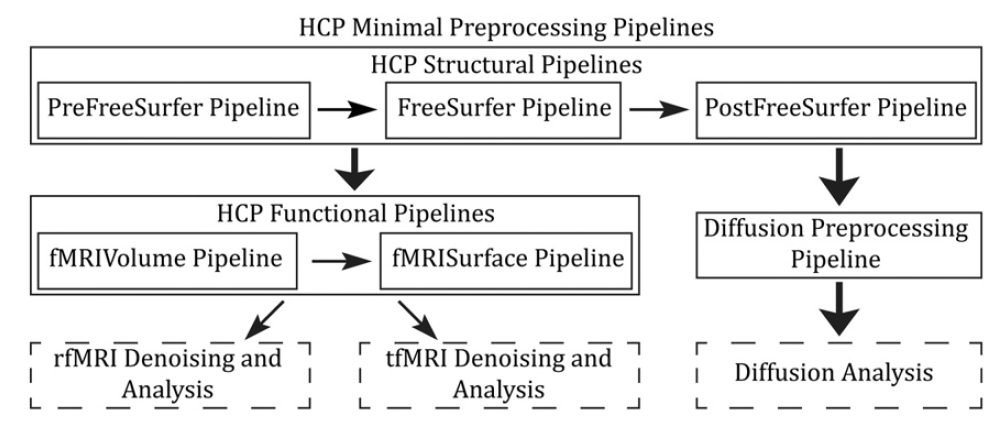
\includegraphics[width=\linewidth]{hcp_preprocessing_overview}
   \captionof{figure}{HCP Preprocessing Pipelines Overview}
   \label{fig:hcp_pipelines_overview}
   \caption*{Extracted from \cite{Gla13}}
\end{center}

Out of the six pipelines illustrated in Figure \ref{fig:hcp_pipelines_overview}, we used three structural pipelines and one functional pipeline for study. The pipelines are listed below,
\begin{itemize}
  \item PreFreeSurfer (Section \ref{sec:PrefreeSurfer})
  \item FreesSurfer   (Section \ref{sec:FreeSurfer})
  \item PostFreeSurfer (Section \ref{sec:PostFreeSurfer})
  \item fMRIVolume    (Section \ref{sec:fMRIVolume})
\end{itemize}

The HCP pipeline is open sourced, and the study is conducted using the version 3.19.0\footnote{\url{https://github.com/Washington-University/Pipelines/releases/tag/v3.19.0}}. The details of pipeines are listed below.

\section{HCP Data} \label{HCP_Data}
HCP Data is collected from a population of adult twins and their non-twin siblings in the age range of 22-35 years. \todo{The previous sentence is a direct quotation} Data from 1200 subjects is available in the ConnectomeDB repository \footnote{\url{https://db.humanconnectome.org/}}. Each HCP data set, is data collected from an individual person and such a directory containing the HCP data is denoted by the term, ``subject". Each subject contains data belonging to four modalities. They are structural MRI, resting-state fMRI (rfMRI), task fMRI (tfMRI), and diffusion MRI (dMRI)~\cite{HCPData}.

\indent Terms ``T1-weighted" and ``T2-weighted" are used quite often in 
the realm of structural images. As per the definition given 
by~\cite{t1w_t2w}, T1-weighted images provides good contrast between 
gray matter and white matter in brain while cerebrospinal fluid is void 
of signal (black color) and T2-weighted images provides good contrast 
between cerebrospinal fluid and brain tissue. \todo{The previous sentence is a direct quotation.} Figures~\ref{fig:T1w} 
and~\ref{fig:T2w} illustrates T1-weighted and T2-weighted images.\\

\begin{center}
  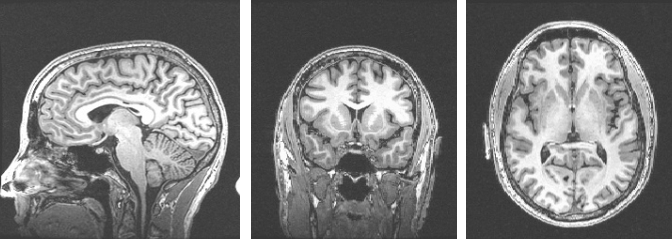
\includegraphics[width=\linewidth]{T1_v3}
  \caption{T1-weighted image}
  \label{fig:T1w}
  \caption*{Extracted from \cite{t1w_t2w}}
\end{center}

\begin{center}
  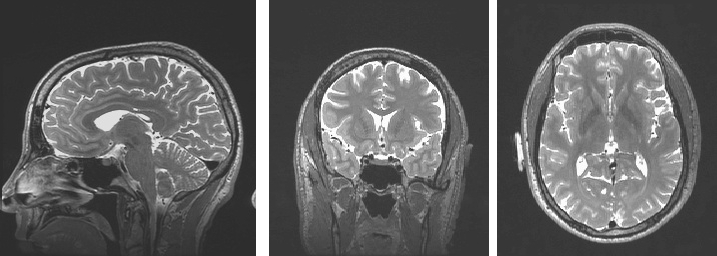
\includegraphics[width=\linewidth]{T2_v1}
  \caption{T2-weighted image}
  \label{fig:T2w}
  \caption*{Extracted from \cite{t1w_t2w}}
\end{center}

\indent Functional data consists of task based and resting state fMRI 
data. Emotion, gambling, language, motor, relational and social are 
examples of task based fMRI data available in the HCP Subjects. Resting 
state data consists of 2 sets (Rest1 and Rest2) in HCP subjects. Task 
based fMRI data is used for studying functional brain networks under 
task performance. Task based fMRI analyses can identify and 
characterize functionally distinct nodes in human 
brain\footnote{\url{https://www.humanconnectome.org/study/hcp-young-adult/project-protocol/resting-state-fmri}}. 
Resting state fMRI consists of data that is collected when the subject 
is not performing an explicit task. This can be used to map the 
regional interactions happening in the brain at the time of 
rest~\footnote{\url{https://www.humanconnectome.org/study/hcp-young-adult/project-protocol/resting-state-fmri}}.


\section{PreFreeSurfer} \label{sec:PrefreeSurfer}
Main goals of PreFreeSurfer, according to~\cite{Gla13} are, ``1) to produce an undistorted ``native" structural volume space for each subject; 2) align the T1W and T2W images; 3) perform bias field correction; 4) register the subject's native structural volume space to MNI space''. The workflow of PreFreeSurfer is illustrated in Figure \ref{fig:prefreesurfer_overview}.

\begin{center}
  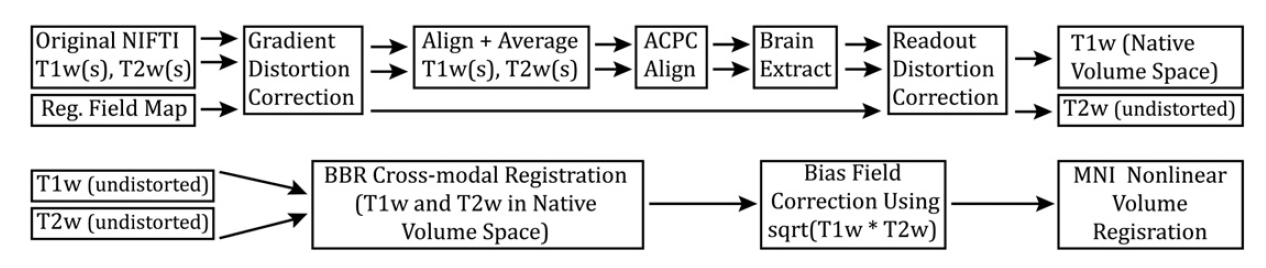
\includegraphics[width=\linewidth]{PreFreeSurfer_Architecture}
  \captionof{figure}{PreFreeSurfer Overview}
  \label{fig:prefreesurfer_overview}
  \caption*{Extracted from \cite{Gla13}}
\end{center}

\indent Figure~\ref{fig:prefreesurfer_overview} illustrates the numbered sequence of steps in the PreFreeSurfer pipeline. The input to the pipeline are T1w and T2w images and the registerted field map. Second step(2) is gradient nonlinearity correction. This distortion is caused by magnetic resonance gradient nonlinearity~\cite{Gla13}. According to~\cite{Zou2004}, ``Gradient nonlinearity is a static characteristic of the gradient coil system known to system engineers and universally utilized for correction of geometric distortions for routine MRI scans''. Gradient nonlinearity distortion must be corrected from all images used for structural preprocessing (T1w, T2w, the field map and phase). Figure~\ref{fig:gradient_nonlinearity} represent gradient nonlinearity distortion correction. Gradient\_nonlin\_unwarp package available in FreeSurfer is used for correcting this distortion. For correcting the gradient nonlinearity distortion, the images are converted into a field map (in units of radians per second) using the fsl\_prepare\_fieldmap\_script. According to \cite{field_map}, ``A field map is an image of the intensity of the magnetic field across space''. Gradient nonlinearity distortion is then corrected with the help of field map. This is followed by warping of the field map magnitude image, according to the readout distortion. Separate registrations of the field map are then done to the T1w and T2w images using FLIRT.

\begin{center}
  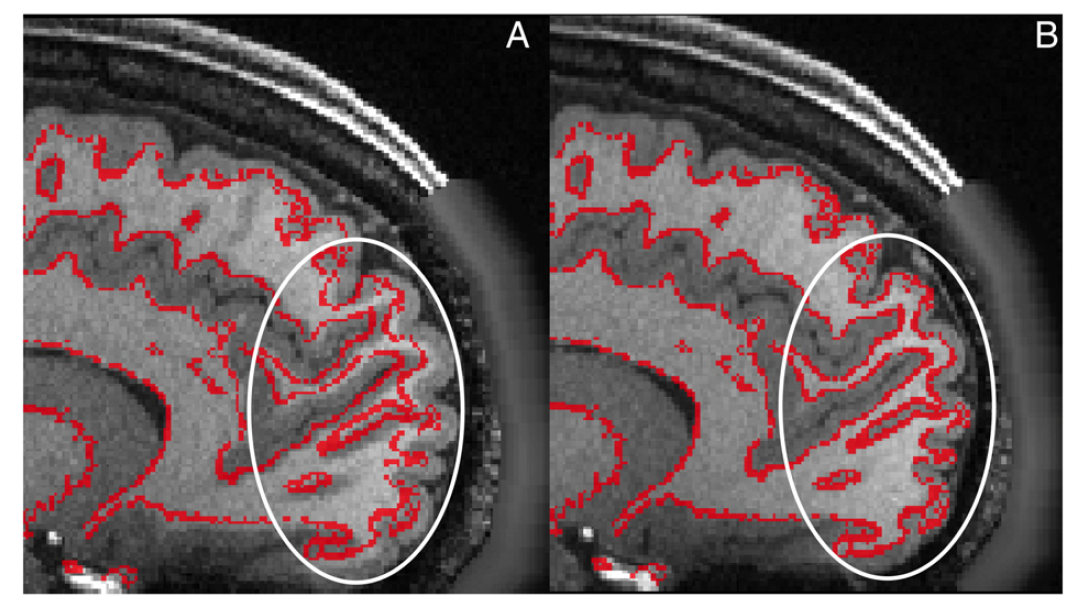
\includegraphics[width=\linewidth]{gradient_nonlinearity_distortion}
  \captionof{figure}[Effect of gradient nonlinearity distortion on the T1w image]{Effect of gradient nonlinearity distortion on the T1w image. Panel A is the T1w image before gradient distortion correction, whereas Panel B is the T1w image after gradient distortion correction}
  \label{fig:gradient_nonlinearity}
  \caption*{Extracted from \cite{Gla13}}
\end{center}
\todo{I think you can remove Figure~\ref{fig:gradient_nonlinearity}, you reused a lot of figures already!}

\indent Next step (3) is aligning the T1w and T2w images, using FSL's FLIRT. Subsequent step is aligning the average T1w and T2w images to the MNI space template. The main purpose behind this step is to have the same orientation as the reference template for the ease of visualization.

\indent Step (4) is ACPC (Anterior commisure, Posterior commisure) alignment. Step (5) includes a robust initial brain extraction, using FSL's linear (FLIRT) and non-linear (FNIRT) registration. Removing the readout distortion is the last step (6) in creating the subject's undistorted native volume space. %Readout distortion is caused when the digital data is retrieved from an electronic medium and is displayed in a human understandable format.
%Readout distortion definition

\indent The distortion corrected images are used as the input for the next series of steps. To completely remove the distortion, the T1w and T2w images are transformed according to of the field map registration. After that, the T1w and T2w images are unwarped, removing the differential readout distortion present in them. The T1w image without readout and spatial distortion, represents the native volume space for each subject.

\indent Step (9) consist of cross-modal registration of undistorted T2w image to the T1w image using FLIRT's boundary based registration (BBR) cost function. Aligning the intensity gradients across tissue boundaries is the focus of boundary based registration. Once T1w and T2w images are in the same space, (10) intensity inhomogeneity correction is applied on these images. After the bias field correction, T1w image is (11) registered to MNI space after a FLIRT registration followed by FNIRT nonlinear registration.

\indent The output of PreFreeSurfer pipeline are organized into a folder called ``T1w" that contains native volume space images and a second folder (MNINonLinear) that contains MNI space images~\cite{Gla13}.

\section{FreeSurfer} \label{sec:FreeSurfer}
HCP pipelines use FreeSurfer version 5.2 with a lot of enhancements made particularly focusing HCP data. The main goals, according to~\cite{Gla13} are, ``1) improve the robustness of brain extraction; 2) fine tune T2w to T1w registration; 3) accurately place the white and pial surface with high resolution data; 4) perform FreeSurfer's standard folding-based surface registration to their surface atlas (fsaverage)''. The workflow of FreeSurfer is illustrated in Figure~\ref{fig:freesurfer_overview}.

\begin{center}
  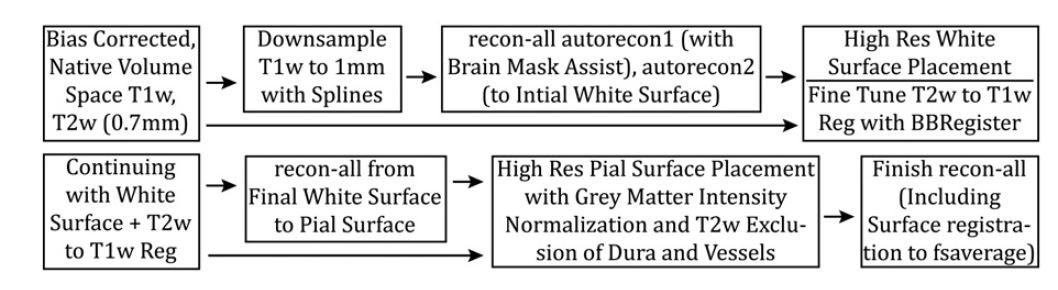
\includegraphics[width=\linewidth]{FreeSurfer_Architecture}
  \captionof{figure}{FreeSurfer Overview}
  \label{fig:freesurfer_overview}
  \caption*{Extracted from \cite{Gla13}}
\end{center}

After the PreFreeSurfer processing, FreeSurfer's recon-all (cortical reconstruction process)\footnote{\url{https://surfer.nmr.mgh.harvard.edu/fswiki/recon-all}} pipeline is used widely in FreeSurfer pipeline. One limitation with the recon-all pipeline is that it is not able to process structural images having high resolution. So HCP data has to be downsampled to meet the requirements of the recon-all pipeline.

The first step (1) in the FreeSurfer pipeline is inputting the disortion and bias free native volume space image from PreFreeSurfer. The T1w registration in the FreeSurfer is aided using the initial brain mask generated in PreFreeSurfer. The important steps that takes place before the recon-all process includes, automated segmentation of the T1w volume and tessellation and topology correction of the initial white matter surface. Also, downsampling of images to a lower resolution takes place at step (2), such that it matches the requirements of recon-all process.

The output of step (3) is white-matter surface created with the help of recon-all process. The resultant white matter surface is generated using a segmentation of the 1 mm downsampled T1w image.

Final white matter surface placement is done with the help of the original high resolution T1w images at step (4). The required FreeSurfer volume and surface files are brought into the .7 mm native volume space and intensity normalization is done on the high resolution T1w image. Also, the white matter surface position is adjusted at those points, where it is placed too superficially into the gray matter, based on intensity gradients in the .7 mm T1w image. The latter part of step (4) handles T2w to T1w registration. This registration step is fine-tuned using FreeSurfer's BBRegister algorithm since it gives more accurate results than FLIRT's BBR implementation. The corrected white matter surfaces are then brought back into FreeSurfer space and recon-all processing resumes.

The set of steps in the FreeSurfer pipeline is for generating the Pial surfaces. The first step (5) in pial surface generation is normalization of T1w and T2w images to a standard mean white matter intensity. The initial pial surfaces are generated (6) from the high-resolution PreFreeSurfer bias-corrected T1w image and not the FreeSurfer white matter specific intensity normalized image. This kind of generation of pial surfaces tend to include large amounts of dura (a thick membrane that is the outermost of the three layers of the meninges that surround the brain and spinal cord) and blood vessels. The dura and blood vessels present in the image are removed (7) with the help of T2w images since dura and blood vessels are very different in intensity from gray matter in the T2w image. Figure \ref{fig:pial_surface_generation} showcases the pial surface generation with the help of T2w images. This initially generated pial surface is smoothened and high pass filtering is done in order to generate the final pial surface.

\begin{center}
  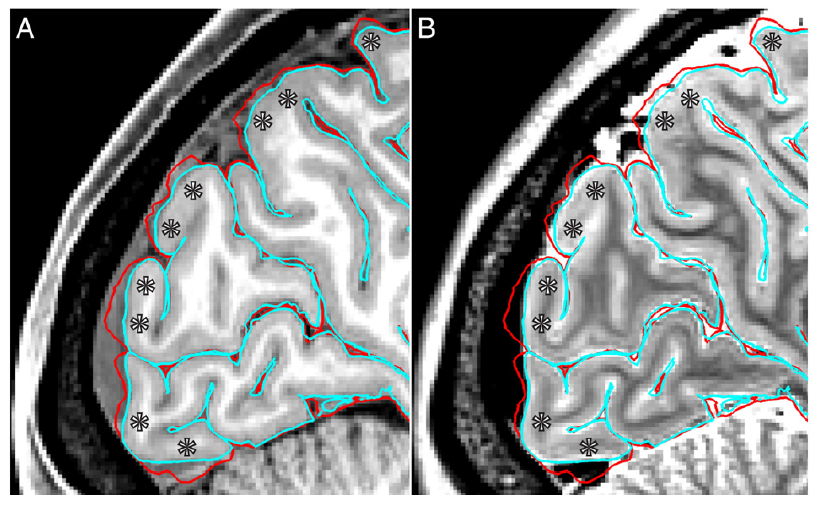
\includegraphics[width=\linewidth]{pial_surface_generation}
  \captionof{figure}[Pial surface generation with the help of T2w image]{Pial surface generation with the help of T2w image. The blood vessels and dura are close in intensity with gray matter in the T1w image (A), however they are clearly of different intensity in the T2w image (B), allowing them to be easily excluded from the gray matter ribbon. The red surface is from the T1w image whereas the cyan surface is after cleanup with the T2w image.}
  \label{fig:pial_surface_generation}
  \caption*{Extracted from \cite{Gla13}}
\end{center}
\todo{Figure~\ref{fig:pial_surface_generation} is again directly extracted. If you want to illustrate the pipeline steps, you should rather use your own images.}

After the pial surface generation, recon-all continues. Final step (8) include anatomical parcellation (surface and volume) and morphometric measurements of structural volumes, surface areas, and thickness.

\section{PostFreeSurfer} \label{sec:PostFreeSurfer}
Main goals of PostFreeSurfer, according to~\cite{Gla13} are, ``1) produces all the NIFTI volume and GIFTI surface files necessary for viewing the data in Connectome Workbench, 2) application of surface registration; According to \cite{DBLP:journals/corr/HrgeticP13}, ''task of the surface registration algorithms is to determine the corresponding surface parts in the pair of observed clouds of 3D points, and on that basis to determine the spatial translation and rotation between the two views"; 3) downsampling registered surfaces for connectivity analyses; 4) creating the final brain mask, and creating myelin maps''. Figure \ref{fig:postfreesurfer_overview} illustrates the workflow of PostFreeSurfer.\\

\begin{center}
  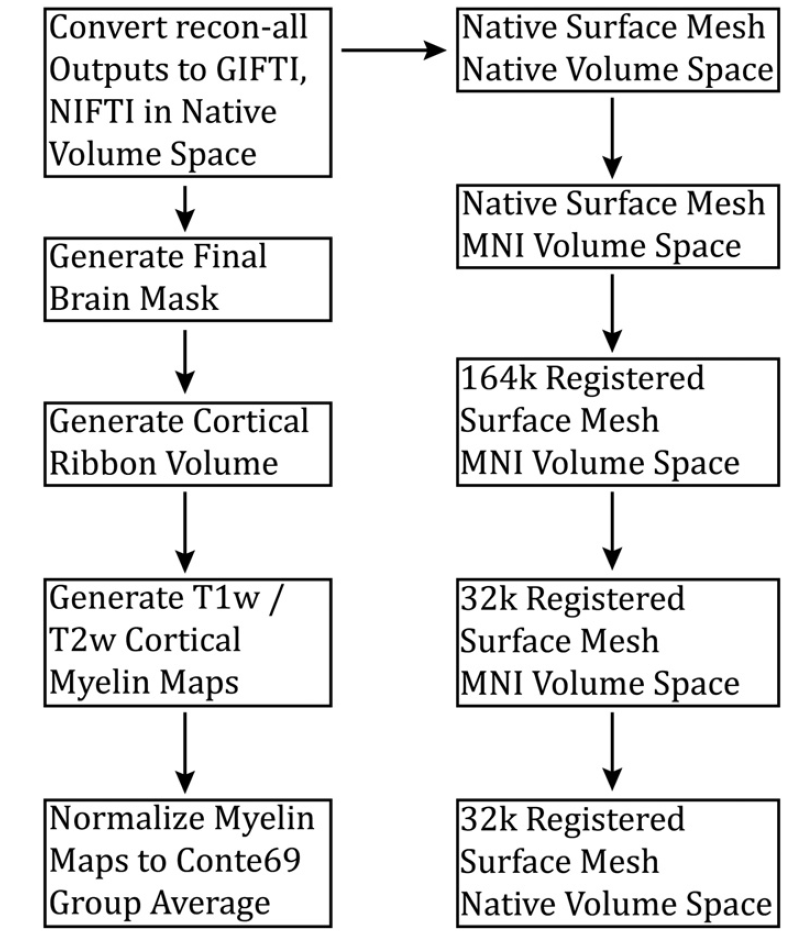
\includegraphics[width=\linewidth]{PostFreeSurfer_Overview}
  \captionof{figure}{PostFreeSurfer Overview}
  \label{fig:postfreesurfer_overview}
  \caption*{Extracted from \cite{Gla13}}
\end{center}

As mentioned in the previous paragraph, the first task (1) of PostFreeSurfer is to convert the recon-all outputs to NIFTI and GIFTI formats. The white, pial, spherical and registered spherical surfaces are all converted GIFTI surface files. Thickness, curvature and sulc files are converted into GIFTI shape files. The cortical parcellations from FreeSurfer are converted to GIFTI label files and three full subcortical volume parcellations are converted into NIFTI label files. One among the three volume parcellations (wmparc) is used to create a final gray and white matter brain mask (2), which is used as the reference in the subsequent steps. Step (3) creates cortical ribbon volume and that step is followed by (4) cortical myelin map creation. Next step (5) is the generation of Conte69 Group Average by normalizing the Myelin Maps. Figure \ref{fig:residual_bias_correction} illustrates the residual bias field correction that takes place in myelin maps.

\begin{center}
  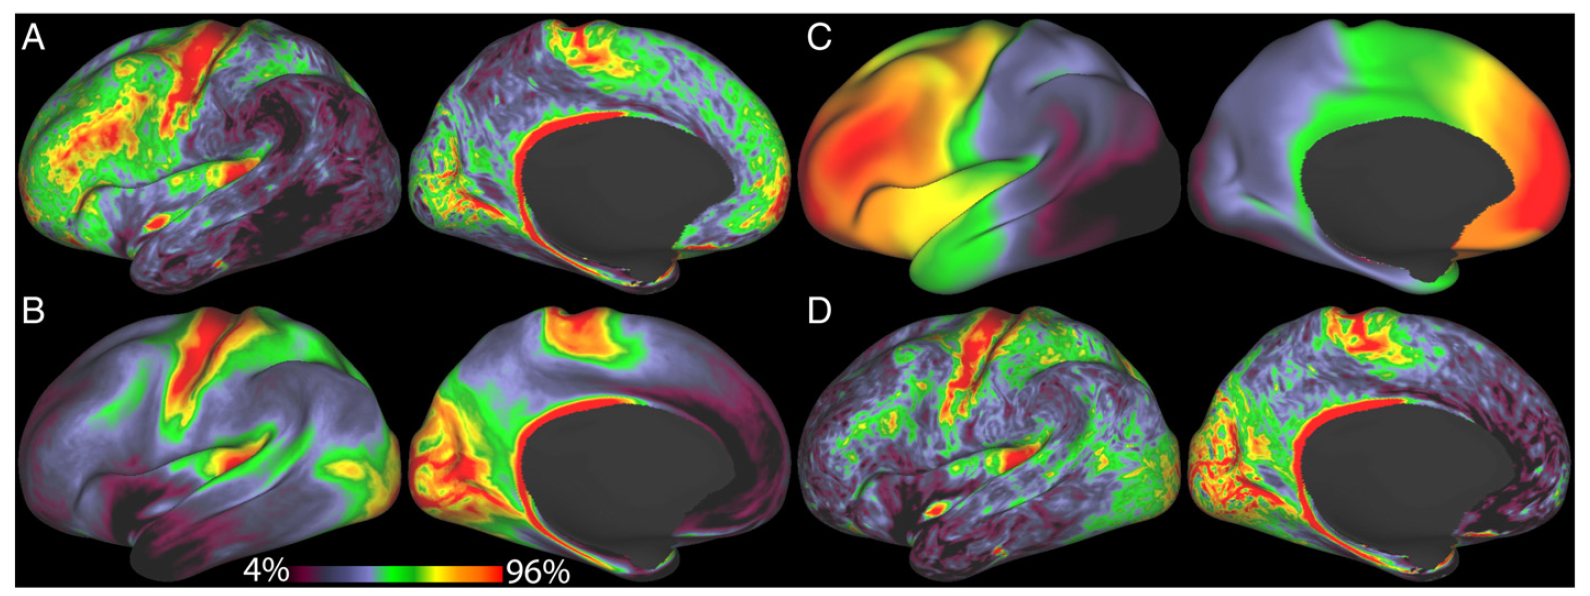
\includegraphics[width=\linewidth]{residual_bias_correction}
  \captionof{figure}[The effect of residual bias field correction]{The effect of residual bias field correction on a particularly inhomogeneous HCP subject. (A) Original Myelin Map. (B) Reference group average myelin map (C) Estimated residual bias field. (D) Bias corrected myelin map.}
  \label{fig:residual_bias_correction}
  \caption*{Extracted from \cite{Gla13}}
\end{center}
\todo{Same comment as before.}

Steps (6-10) leads to the creation of 32k Registered Surface Mesh Native Volume Space. It starts off with step (6) where the pipeline combines the structural transforms of T1w and T2w images from the PreFreeSurfer and FreeSurfer pipelines. This transformed file is then applied to the averaged T1w and T2w images, and they are brought to the native volume and MNI spaces. Next step is creating a mid-thickness surface. It is created by averaging the white and pial surfaces. Mid-thickness file is used for creating inflated and very inflated files. The volume, label and metric files are then organized into a file called as specification file (spec file) which is used for easy visualization of anatomical data using Connectome Workbench. The surface files are stored as GIFTI files while the specs files are CIFTI files.

Step (7) uses the Conte69\footnote{\url{http://brainvis.wustl.edu/wiki/index.php//Caret:Atlases/Conte69\_Atlas}} (Human Surface-based Atlas and Reference Data) population-average surfaces for registering individual subject's native-mesh surfaces. This step consists of combined surface registration applied to all surfaces and surface data files. The end goal of this step is to bring the images to (8) 164k\_fs\_LR standard surface mesh space.

Registration step is followed by (9) the downsampling of the 164k Registered surface mesh to 32k\_fs\_LR MNI volume space. These lower resolution images are suited for functional and connectivity analyses. The last step (10) in this pipeline is transformation of the 32k\_fs\_LR mesh from MNI space to native volume space.

%Specification File (commonly called “Spec File”) is a file used to organize a set of data files (such as volume, label, and metric files) to be loaded into Workbench

\section{fMRIVolume} \label{sec:fMRIVolume}
Main goals of, fMRIVolume, according to~\cite{Gla13} are, ``1) remove spatial distortions; 2) realignment of volumes to adjust subject motion; 3) registration of fMRI data to structural volume; 4) normalizaton of the 4D image; 5) mask the data with final brain mask''. Figure \ref{fig:fMRIVolume_overview} illustrates the workflow of fMRIVolume pipeline.

It is a prerequisite of fMRIVolume pipeline that the input files should have completed the structural processing (PreFreeSurfer, FreeSurfer and PostFreeSurfer). Similiar to the PreFreeSurfer pipeline, fMRIVolume pipeline starts with the gradient-nonlinearity-induced distortion correction step (2), though it is optional. It is followed by (3) subject motion correction using FLIRT. The distortion in the phase encoding direction is corrected in the next step (4). In the next step (5), with the use of FLIRT, BBR cost function and FreeSurfer's BBRegister, an accurate registration between fMRI data and the structural data is created. The final step (8) in the fMRIVolume pipeline consists of concatenating all the transforms for each registration and distortion correction into a single nonlinear transformation.

\begin{center}
  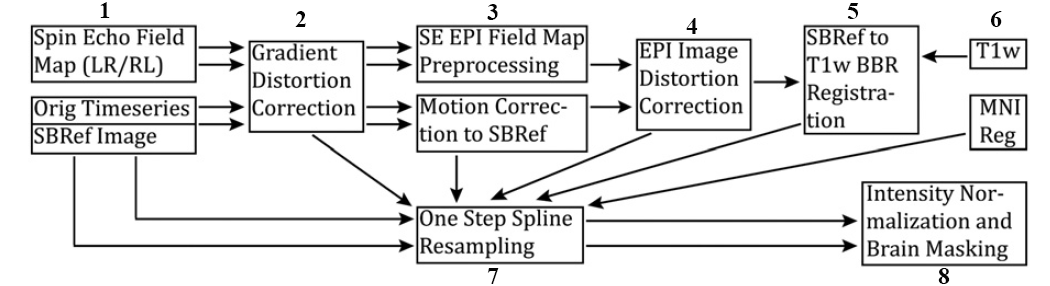
\includegraphics[width=\linewidth]{fMRI_Volume}
  \captionof{figure}{fMRI Volume Overview}
  \label{fig:fMRIVolume_overview}
  \caption*{Extracted from \cite{Gla13}}
\end{center}

\section{Subjects used for the study}\label{subjects_used}
\subsection{HCP Data Selection}
The data was obtained from Human Connectome Project\footnote{\url{https://db.humanconnectome.org}}. We used the subjects 101006, 101017, 101410, 104820 and 105216. All these subjects were scanned using the HCP3T type of scanner. Tables \ref{tab:hcp_subject_details} and \ref{tab:subject_scan_details} give more insight about the HCP subjects that were used for our study.

\begin{center}
\tabulinesep=1.2mm
\begin{tabu} to \textwidth { | X[l] | X[l] | X[l] | X[l] | X[l] | }
  \hline
  Subject & Release & Acquisition & Gender & Age \\
  \hline
  101006 & S500 & Q06 & F & 31-35 \\
  \hline
  101107 & S500 & Q06 & M & 22-25 \\
  \hline
  101410 & S500 & Q06 & M & 26-30 \\
  \hline
  104820 & S500 & Q06 & F & 36+ \\
  \hline
  105216 & Q3 & Q03 & M & 26-30 \\
  \hline
\end{tabu}
\captionof{table}{HCP Subject Details}
\caption*{Data retrieved from \cite{DBConnectomeSite}}
\label{tab:hcp_subject_details}
\end{center}

\begin{center}
\tabulinesep=1.2mm
\begin{tabu} to \textwidth { | X[l] | X[l] | }
  \hline
  Subject ID & Size \\
  \hline
  101006 & 12.4 GB \\
  \hline
  101107 & 12.5 GB \\
  \hline
  101410 & 7.5  GB \\
  \hline
  104820 & 7.2  GB \\
  \hline
  105216 & 14.4 GB \\
  \hline
\end{tabu}
\captionof{table}{Unprocessed HCP Subject Size}
\label{tab:hcp_subject_size}
\end{center}

\begin{center}
  \begin{longtabu} to \textwidth{ | X[l] | X[l] | X[l] | X[l] | }
  \hline
  Subject & MR Session Scanner 3T & MR Session Scans 3T & MR Session Label 3T \\
  \hline
  101006 & HCP 3T & Bias Receive(8), Bias Transmit(1), dMRI(6), dMRI SBRef(6), FieldMap(2), FieldMap SE EPI(8), rfMRI(4), rfMRI SBRef(4), T1w(2), T2w(2), tFMRI(14), tfMRI SBRef(14) & 101006 3T \\
  \hline
  101107 & HCP 3T & Bias Receive(8), Bias Transmit(1), dMRI(6), dMRI SBRef(6), FieldMap(2), FieldMap SE EPI(8), rfMRI(4), rfMRI SBRef(4), T1w(2), T2w(2), tFMRI(14), tfMRI SBRef(14) & 101107 3T \\
  \hline
  101410 & HCP 3T & Bias Receive(10), Bias Transmit(1), dMRI(6), dMRI SBRef(6), FieldMap(2), FieldMap SE EPI(6), rfMRI(2), rfMRI SBRef(2), T1w(2), T2w(1), tFMRI(14), tfMRI SBRe(14) & 101410 3T \\
  \hline
  104820 & HCP 3T & Bias Receive(8), Bias Transmit(1), dMRI(6), dMRI SBRef(6), FieldMap(2), FieldMap SE EPI(8), rfMRI(4), rfMRI SBRef(4), T1w(1), T2w(1), tFMRI(14), tfMRI SBRef(14) & 104820 3T\\
  \hline
  105216 & HCP 3T & Bias Receive(8), Bias Transmit(1), dMRI(6), dMRI SBRef(6), FieldMap(2), FieldMap SE EPI(8), rfMRI(4), rfMRI SBRef(4), T1w(2), T2w(2), tFMRI(14), tfMRI SBRef(14) & 105216 3T\\
  \hline
\caption{Subject Scan Details}
\label{tab:subject_scan_details}
\end{longtabu}
\caption*{Data retrieved from \cite{DBConnectomeSite}}
\end{center}

\section{HCP Docker Images}\label{hcp_docker}
We conducted our study across Docker containers created out of CentOS 6.8 and CentOS 7.2.1511. CentOS\footnote{\url{https://en.wikipedia.org/wiki/CentOS}} (Community Enterprise Operating System) according to~\cite{CentOS}, is a widely used operating system among the Neuroscience community. CentOS operating system is widely known for the community support, network functions, safety, portability and openness~\cite{5665431}. All these qualities make CentOS a popular choice among the research community and high performance computing clusters.
These containers were installed with all the necessary softwares and libraries required to run the HCP pipelines. HCP pipelines prerequisites are listed below,
\begin{itemize}
\item A 64-bit Linux Operating System
\item FSL Version - 5.0.6
\item FreeSurfer Version - 5.3.0-HCP
\item Connectome Workbench Version - 1.0
\item HCP version of gradunwarp version 1.0.2 (this is optional and needs to be installed only if gradient nonlinearity corrections needs to be done)
\end{itemize}
FSL 5.0.6\footnote{\url{https://fsl.fmrib.ox.ac.uk/fsldownloads/oldversions/}}, FreeSurfer 5.3.0-HCP\footnote{\url{http://ftp.nmr.mgh.harvard.edu/pub/dist/freesurfer/5.3.0-HCP/}} (CentOS 4 build) and Connectome Workbench 1.0\footnote{\url{https://www.humanconnectome.org/software/get-connectome-workbench}} were installed in the containers with the help of DockerFiles.
Docker container creation was automated with the help of GitHub and DockerHub. All the containers that are used for this study are available in the Dockerhub\footnote{\url{https://hub.docker.com/r/bigdatalabteam/hcp-prefreesurfer/tags/}}.

\section{Processing of subjects} \label{processing_subjects}
The data was processed in the order PreFreeSurfer, FreeSurfer, PostFreeSurfer and fMRIVolume. Two runs were made on CentOS6 and CentOS7 using the five subjects listed in Table ~\ref{tab:hcp_subject_size}.
\subsection{PreFreeSurfer}
Table \ref{tab:prefreesurfer_processing_details} contains the details about processing time and file-size on CentOS6 and CentOS7 respectively.
Average time taken for PreFreeSurfer processing is 73.7 minutes (10 runs) and average output file size of PreFreeSurfer processing is 13.08 GB (5 subjects) on CentOS6.
Average time taken for PreFreeSurfer processing is 80.2 minutes (10 runs) and average output file size of PreFreeSurfer processing is 13.10 GB (5 subjects) on CentOS7.

\begin{center}
\tabulinesep=1.2mm
\begin{tabular}{ | l | l | l | }
  \hline
    \textbf{Condition} & \textbf{Average Time} & \textbf{Average File Size} \\
  \hline
    CentOS 6 & 73.7 min. & 13.08 GB \\
  \hline
    CentOS 7 & 80.2 min. & 13.10 GB \\
  \hline
\end{tabular}
\captionof{table}{PreFreeSurfer processing details}
\label{tab:prefreesurfer_processing_details}
\end{center}

%\begin{center}
%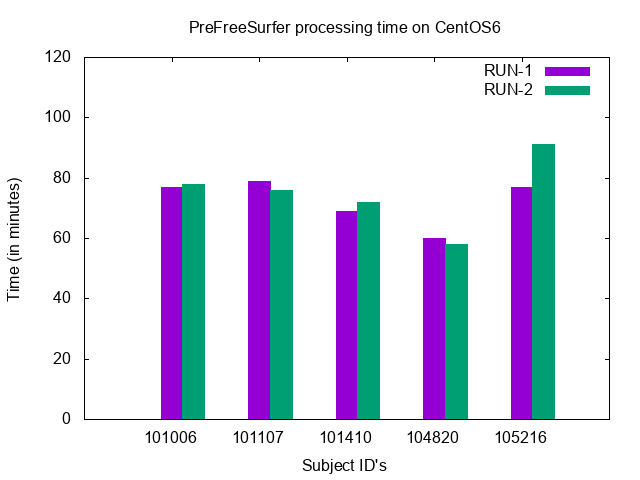
\includegraphics[width=.5\linewidth]{prefreesurfer_run_CentOS6.png}%
%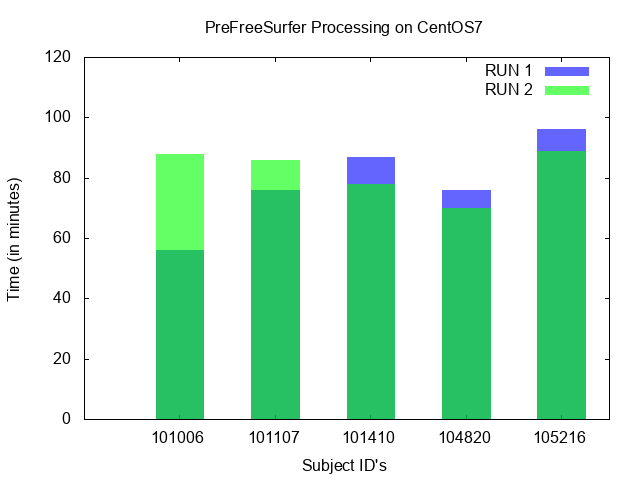
\includegraphics[width=.5\linewidth]{prefreesurfer_run_CentOS7.png}
%\captionof{figure}{PreFreeSurfer processing times }
%\caption*{(i) CentOS6 (left) (ii)CentOS7 (right)}
%\label{fig:prefreesurfer_run}
%\end{center}

%\begin{center}
%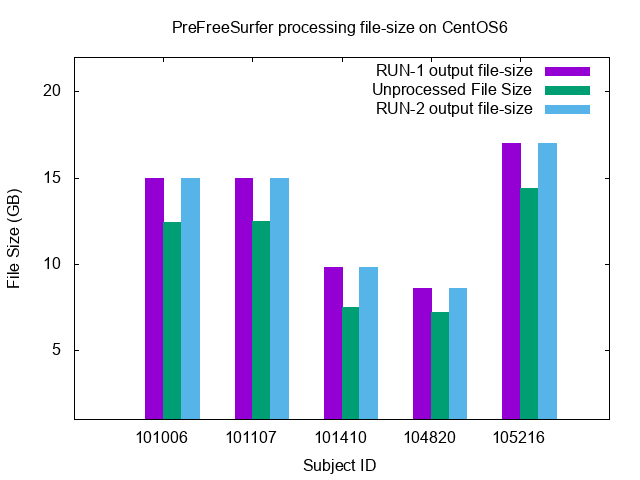
\includegraphics[width=.5\linewidth]{prefreesurfer_CentOS6_filesize.png}%
%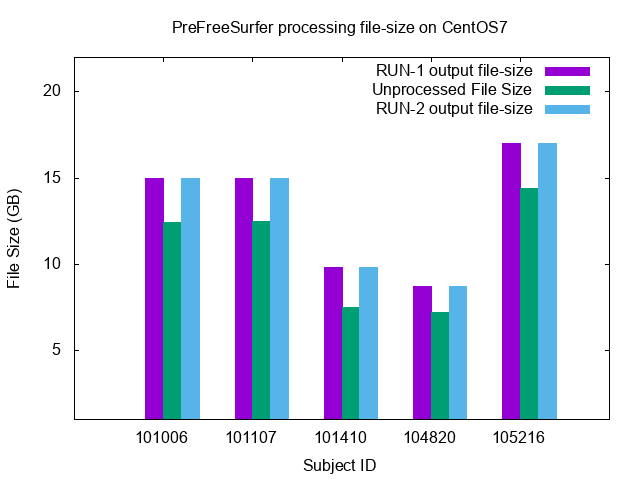
\includegraphics[width=.5\linewidth]{prefreesurfer_CentOS7_filesize.png}
%\captionof{figure}{PreFreeSurfer processing file-sizes}
%\caption*{(i) CentOS6 (left) (ii)CentOS7 (right)}
%\label{fig:prefreesurfer_file_size}
%\end{center}

\subsection{FreeSurfer}
Table \ref{tab:freesurfer_processing_details} contains the details about processing time and file-size on CentOS6 and CentOS7 respectively.
Average time taken for FreeSurfer processing is 7.4 hours (10 runs) and average output file size of FreeSurfer processing is 15.2 GB (5 subjects) on CentOS6.
Average time taken for FreeSurfer processing is 7.58 hours (10 runs) and average output file size of FreeSurfer processing is 15.2 GB (5 subjects) on CentOS7.

\begin{center}
\begin{tabular}{ | l | l | l | }
  \hline
    \textbf{Condition} & \textbf{Average Time} & \textbf{Average File Size} \\
  \hline
    CentOS 6 & 7.4 hours & 15.2 GB \\
  \hline
    CentOS 7 & 7.58 hours & 15.2 GB \\
  \hline
\end{tabular}
\captionof{table}{FreeSurfer processing details}
\label{tab:freesurfer_processing_details}
\end{center}

%\begin{center}
%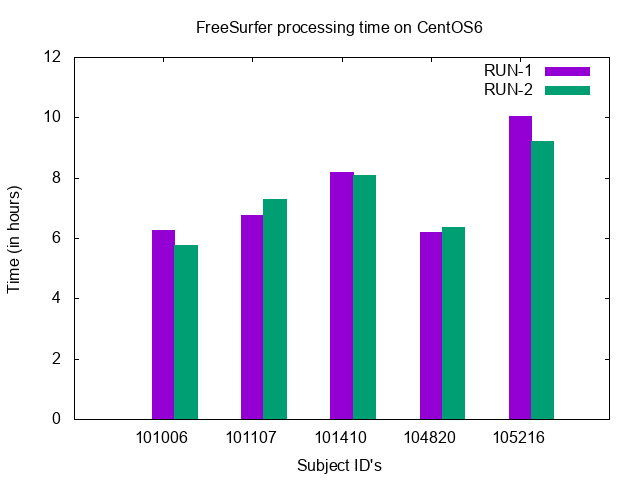
\includegraphics[width=.5\linewidth]{freesurfer_run_CentOS6.png}%
%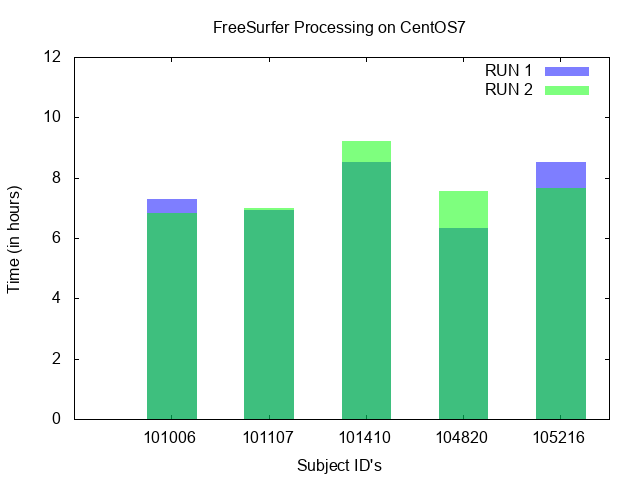
\includegraphics[width=.5\linewidth]{freesurfer_run_CentOS7.png}
%  \captionof{figure}{FreeSurfer processing times}
%  \caption*{(i) CentOS6 (left) (ii)CentOS7 (right)}
%\label{fig:freesurfer_run}
%\end{center}

%\begin{center}
%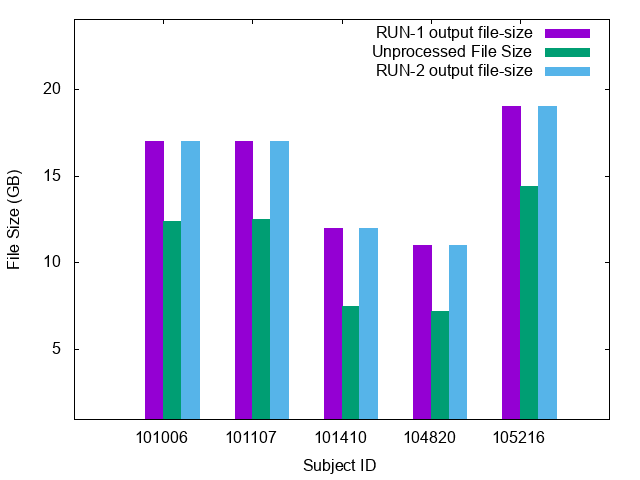
\includegraphics[width=.5\linewidth]{freesurfer_CentOS6_filesize.png}%
%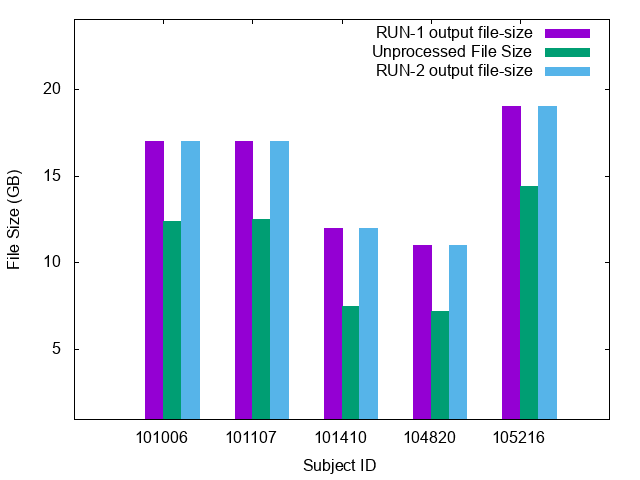
\includegraphics[width=.5\linewidth]{freesurfer_CentOS7_filesize.png}
%  \captionof{figure}{FreeSurfer processing file-sizes}
%  \caption*{(i) CentOS6 (left) (ii)CentOS7 (right)}
%\label{fig:freesurfer_file_size}
%\end{center}

\subsection{PostFreeSurfer}
Table \ref{tab:postfreesurfer_processing_details} contains the details about processing time and file-size on CentOS6 and CentOS7 respectively.
Average time taken for FreeSurfer processing is 22.5 minutes (10 runs) and average output file size of FreeSurfer processing is 16.2 GB (5 subjects) on CentOS6.
Average time taken for FreeSurfer processing is 28.3 minutes (10 runs) and average output file size of FreeSurfer processing is 16.2 GB (5 subjects) on CentOS7.

\begin{center}
\begin{tabular}{ | l | l | l | }
  \hline
    \textbf{Condition} & \textbf{Average Time} & \textbf{Average File Size} \\
  \hline
    CentOS 6 & 22.5 min. & 16.02 GB \\
  \hline
    CentOS 7 & 28.3 min. & 16.02 GB \\
  \hline
\end{tabular}
\captionof{table}{PostFreeSurfer processing details}
\label{tab:postfreesurfer_processing_details}
\end{center}

%\begin{center}
%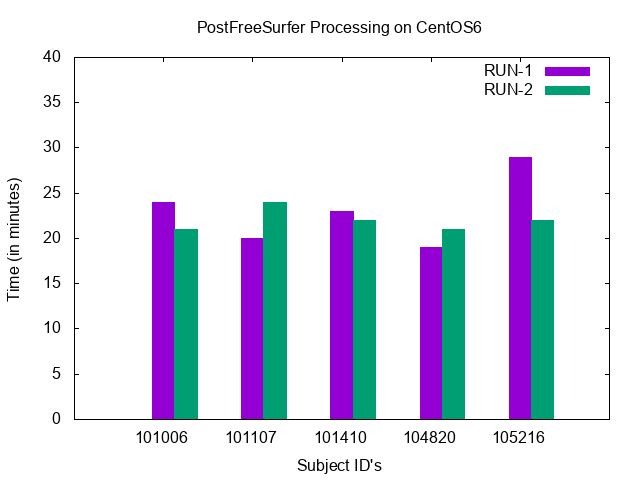
\includegraphics[width=.5\linewidth]{postfreesurfer_run_CentOS6.png}%
%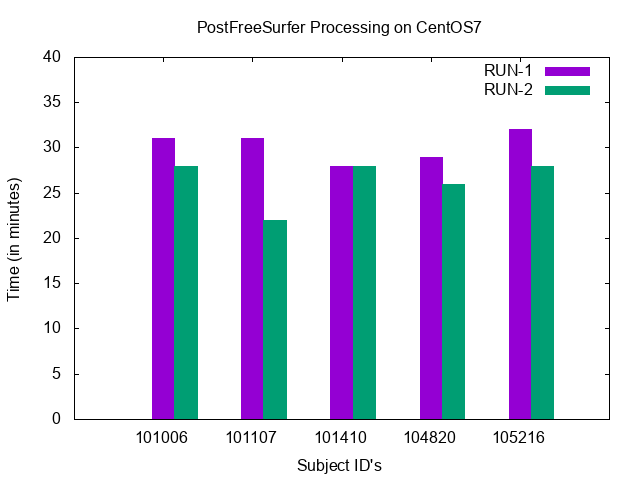
\includegraphics[width=.5\linewidth]{postfreesurfer_run_CentOS7.png}
%\captionof{figure}{PostFreeSurfer processing times}
%\caption*{(i) CentOS6 (left) (ii)CentOS7 (right)}
%\label{fig:postfreesurfer_run}
%\end{center}

%\begin{center}
%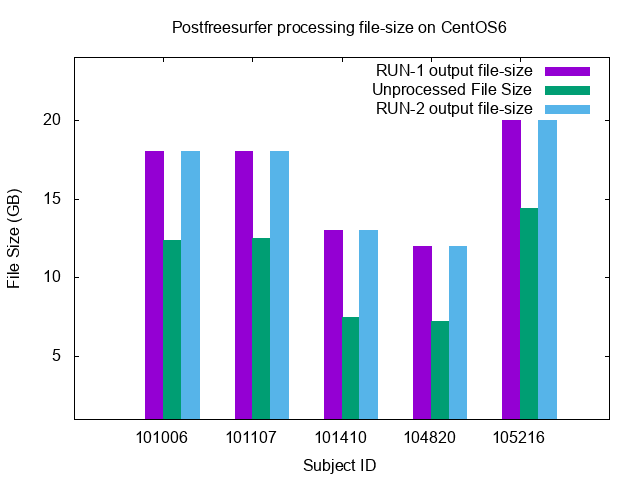
\includegraphics[width=.5\linewidth]{postfreesurfer_CentOS6_filesize.png}%
%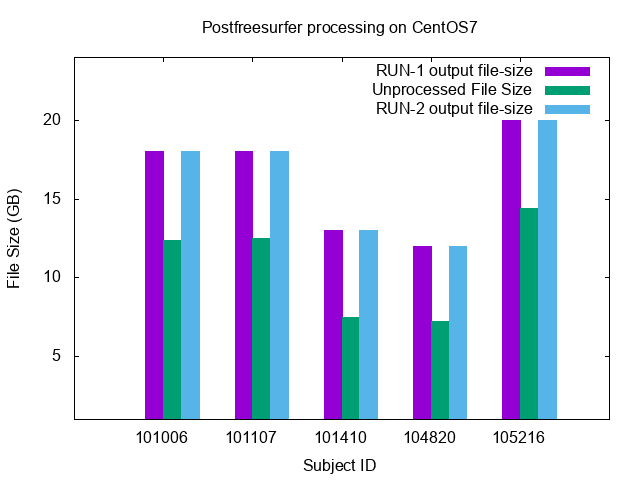
\includegraphics[width=.5\linewidth]{postfreesurfer_CentOS7_filesize.png}
%\captionof{figure}{PostFreeSurfer processing file-sizes}
%\caption*{(i) CentOS6 (left) (ii)CentOS7 (right)}
%\label{fig:postfreesurfer_file_size}
%\end{center}

\subsection{fMRIVolume}
Table \ref{tab:fmrivolume_processing_details} contains the details about processing time and file-size on CentOS6 and CentOS7 respectively.
Average time taken for FreeSurfer processing is 24.68 hours (10 runs) and average output file size of FreeSurfer processing is 221.2 GB (10 subjects) on CentOS6.
Average time taken for FreeSurfer processing is 24.76 hours (10 runs) and average output file size of FreeSurfer processing is 220.8 GB (10 subjects) on CentOS7.

\begin{center}
\begin{tabular}{ | l | l | l | }
  \hline
    \textbf{Condition} & \textbf{Average Time} & \textbf{Average File Size} \\
  \hline
    CentOS 6 & 24.68 hours & 221.2 GB \\
  \hline
    CentOS 7 & 24.76 hours & 220.8 GB \\
  \hline
\end{tabular}
\captionof{table}{fMRIVolume processing details}
\label{tab:fmrivolume_processing_details}
\end{center}

%\begin{center}
%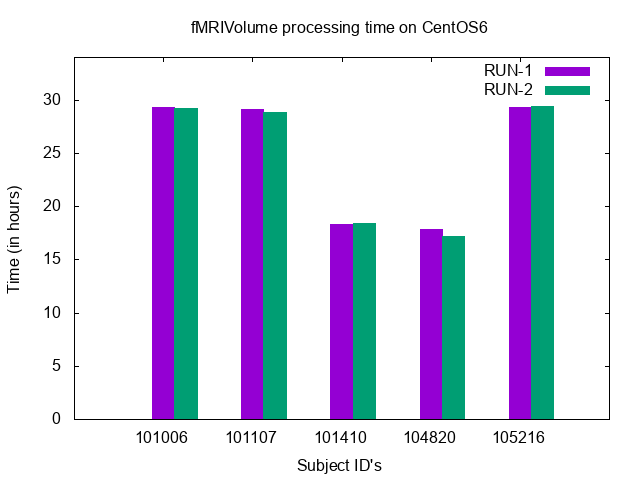
\includegraphics[width=.5\linewidth]{fmri_run_CentOS6.png}%
%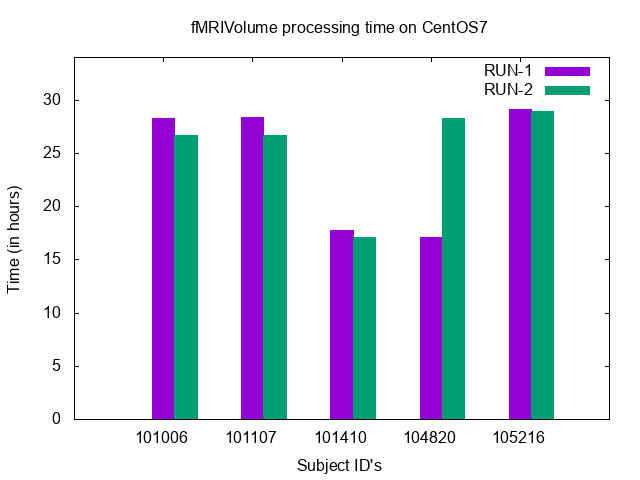
\includegraphics[width=.5\linewidth]{fmri_run_CentOS7.png}
%\captionof{figure}{fMRIVolume processing times}
%\caption*{(i) CentOS6 (left) (ii)CentOS7 (right)}
%\label{fig:fmri_run}
%\end{center}

%\begin{center}
%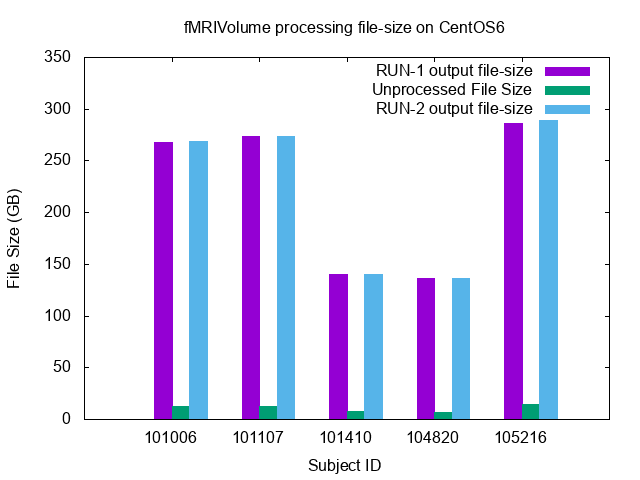
\includegraphics[width=.5\linewidth]{fmri_CentOS6_filesize.png}%
%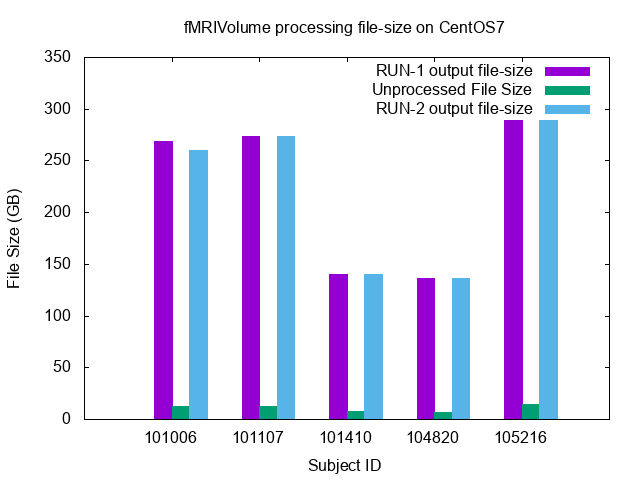
\includegraphics[width=.5\linewidth]{fmri_CentOS7_filesize.png}
%\captionof{figure}{fMRIVolume processing file-sizes}
%\caption*{(i) CentOS6 (left) (ii)CentOS7 (right)}
%\label{fig:fmri_file_size}
%\end{center}

